\documentclass[11pt]{article}
\usepackage[margin=1in]{geometry}
\usepackage{amsfonts, amsmath, amssymb}
\usepackage{mhchem}
\usepackage{parskip}
\usepackage{graphicx}
\graphicspath{.}
\usepackage{subcaption}
\usepackage{placeins}
\usepackage[utf8]{inputenc} 
\usepackage[T1]{fontenc} 
\usepackage{mathpazo} % Palatino font
\usepackage[backend=biber,style=apa]{biblatex}
\addbibresource{{~/Zotero/Zotero.bib}}
\usepackage{fancyhdr}
\usepackage{pdfpages}
\usepackage{hyperref}

\pagestyle{fancy}
\fancyhead{}
\fancyfoot{}
\fancyhead[L]{\MakeUppercase{CHEM3003}}
\fancyhead[R]{\thepage}
\fancyfoot[L]{\textit{Aaron Copeland} | 19765288}
\setlength{\parindent}{0pt}

\begin{document}

\begin{titlepage} 
\newcommand{\HRule}{\rule{\linewidth}{0.5mm}} 
	
	\center % Centre everything on the page

	
	\textsc{\LARGE Curtin University}\\[1.5cm] % Main heading such as the name of your university/college
	
	\textsc{\Large Research, Leadership and Entrepreneurship in Science 2}\\[0.5cm] % Major heading such as course name
	
	\textsc{\large NPSC3000}\\[0.5cm] % Minor heading such as course title
	
	\HRule\\[0.4cm]
	
	{\huge\bfseries Portfolio}\\[0.4cm] % Title of your document
	
	\HRule\\[1.5cm]
	
	\begin{minipage}{0.5\textwidth}
		\begin{flushleft}
			\large
			\textit{Author}\\
			A.D. \textsc{Copeland}\\
                        \textit{ID}: 19765288\\
                        \textit{Email}: \texttt{19765288@student.curtin.edu.au}\\
                        \textit{Due Date}: 29 September 2023
		\end{flushleft}
	\end{minipage}
	~
	\begin{minipage}{0.4\textwidth}
		\begin{flushright}
			\large
			\textit{Unit Coordinator}\\
			Assoc. Prof. Katarina \textsc{Miljkovic}\\ % Supervisor's name
		\end{flushright}
	\end{minipage}
	
	% If you don't want a supervisor, uncomment the two lines below and comment the code above
	%{\large\textit{Author}}\\
	%John \textsc{Smith} % Your name
	
	%------------------------------------------------
	%	Date
	%------------------------------------------------

	\vfill\vfill % Position the date 3/4 down the remaining page

    \raggedright
    
	\large\today % Date, change the \today to a set date if you want to be precise
	
\end{titlepage}

\section{Reflections}

\subsection{Finding a Workflow}

A lot of my project revolves around using a terminal emulator and command line tools on my laptop to set up and run simulations via a remote computer using the \texttt{ssh} protocol. I am very familiar and capable with using these kinds of tools from previous experience, both for university and personal work. I found that using command line tools to view, move and modified files to become a hassle when trying to set up a new directory for a new kind of simulation. It's important that I can do this on the command line, but it didn't gel with me - it didn't feel smooth. It felt sort of like, make a directory, change into it, copy a file from the old directory, enter a text-editor to change the file, exit the editor, make a new file, and so on... These are usually all seperate commands, so the process can feel jarring. Emacs to the rescue! I've been using the text-editor, development environment, Emacs, over the last year for various things like document creation and programming. For setting up and running simulations for my project, Emacs was somewhat of an alternative to just using a terminal emulator. Using the \href{https://www.emacswiki.org/emacs/TrampMode}{TRAMP} package that is built into emacs, I was able to connect to a remote machine and use the directory editor of emacs as a more graphical way for organising my simulation files - it's a bit more like using a traditional file manager on a computer. Instead of having to use a text-editor inside of the terminal to make changes to files, I can view and edit them directly from inside Emacs with my same configuration that I use for editing local files on my machine. What about queuing and running a simulation? Simple. I can open up a shell for the remote machine in a seperate space within Emacs and use the necessary command line tools there (have a look at Figure~\ref{fig:emacs-refl}). I really like that I can do all of this from within a program that I have set up with key-bindings and settings that suit my workflow. I make sure I am proficient with using common tools like the terminal and command line, but I feel more productive using something like Emacs to make tasks suit how I work best.

\begin{figure}[h!]
  \centering
  \includegraphics[height=6cm]{graphics/emacs-refl}
  \caption{My usual working environment in Emacs. The top left section is the directory editor, the bottow left is a shell, and the right section is a file I am editing.}
  \label{fig:emacs-refl}
\end{figure}

\subsection{Pawsey Tour}

On Thursday March 30th the Curtin Computational Chemistry group, along with three visiting Italian Masters students, toured the Pawsey supercomputing facility in Technology Park near the Curtin University Campus. The visiting students were being introduced to the prospect of studying a PhD in Australia and shown what Curtin has to offer. I found it valuable chatting with these students. They seemed open to the idea of completing a PhD in Australia, Perth specifically. They liked our mild weather and location. I think the location of study is important in reinforcing positive learning and feeling towards studying. I haven't properly considered studying or working overseas. I'm definitely not opposed to it, but chatting with the students has made me conscious that I need to consider the town and surrounds of a possible place I might move to. I have ideas about countries that I would like to study in, but countries are so vast in culture, climate and people that I now know I have to be specific in my search for a host town or city (if or when I choose to look seriously at overseas study!).

The tour started with a presentation about the history and current specifications of the Pawsey supercomputers and the precinct itself. This was a fairly generic presentation, but interesting nonetheless. I was particularly intrigued by the centers used of an underground aquifer to aid in water-cooling the supercomputers. This is an ingenious way of reducing grid power requirements for the supercomputers. I can tell that a lot of planning went into developing the Pawsey center. After this we got to peer through the windows to where the supercomputers (and a small quantum computer) were housed. Figure~\ref{fig:pawsey} shows a photograph of my view. While the supercomputers are much larger than any other computer I've seen in person, they also appeared quite small. A few students on the tour gave a small snicker upon seeing it for the first time. I suppose we were expecting an super-sized computer! I'm somewhat glad at seeing how compact the system was, given its power output (and power requirements). It is an impressive feat of engineering.

\begin{figure}[h!]
  \centering
  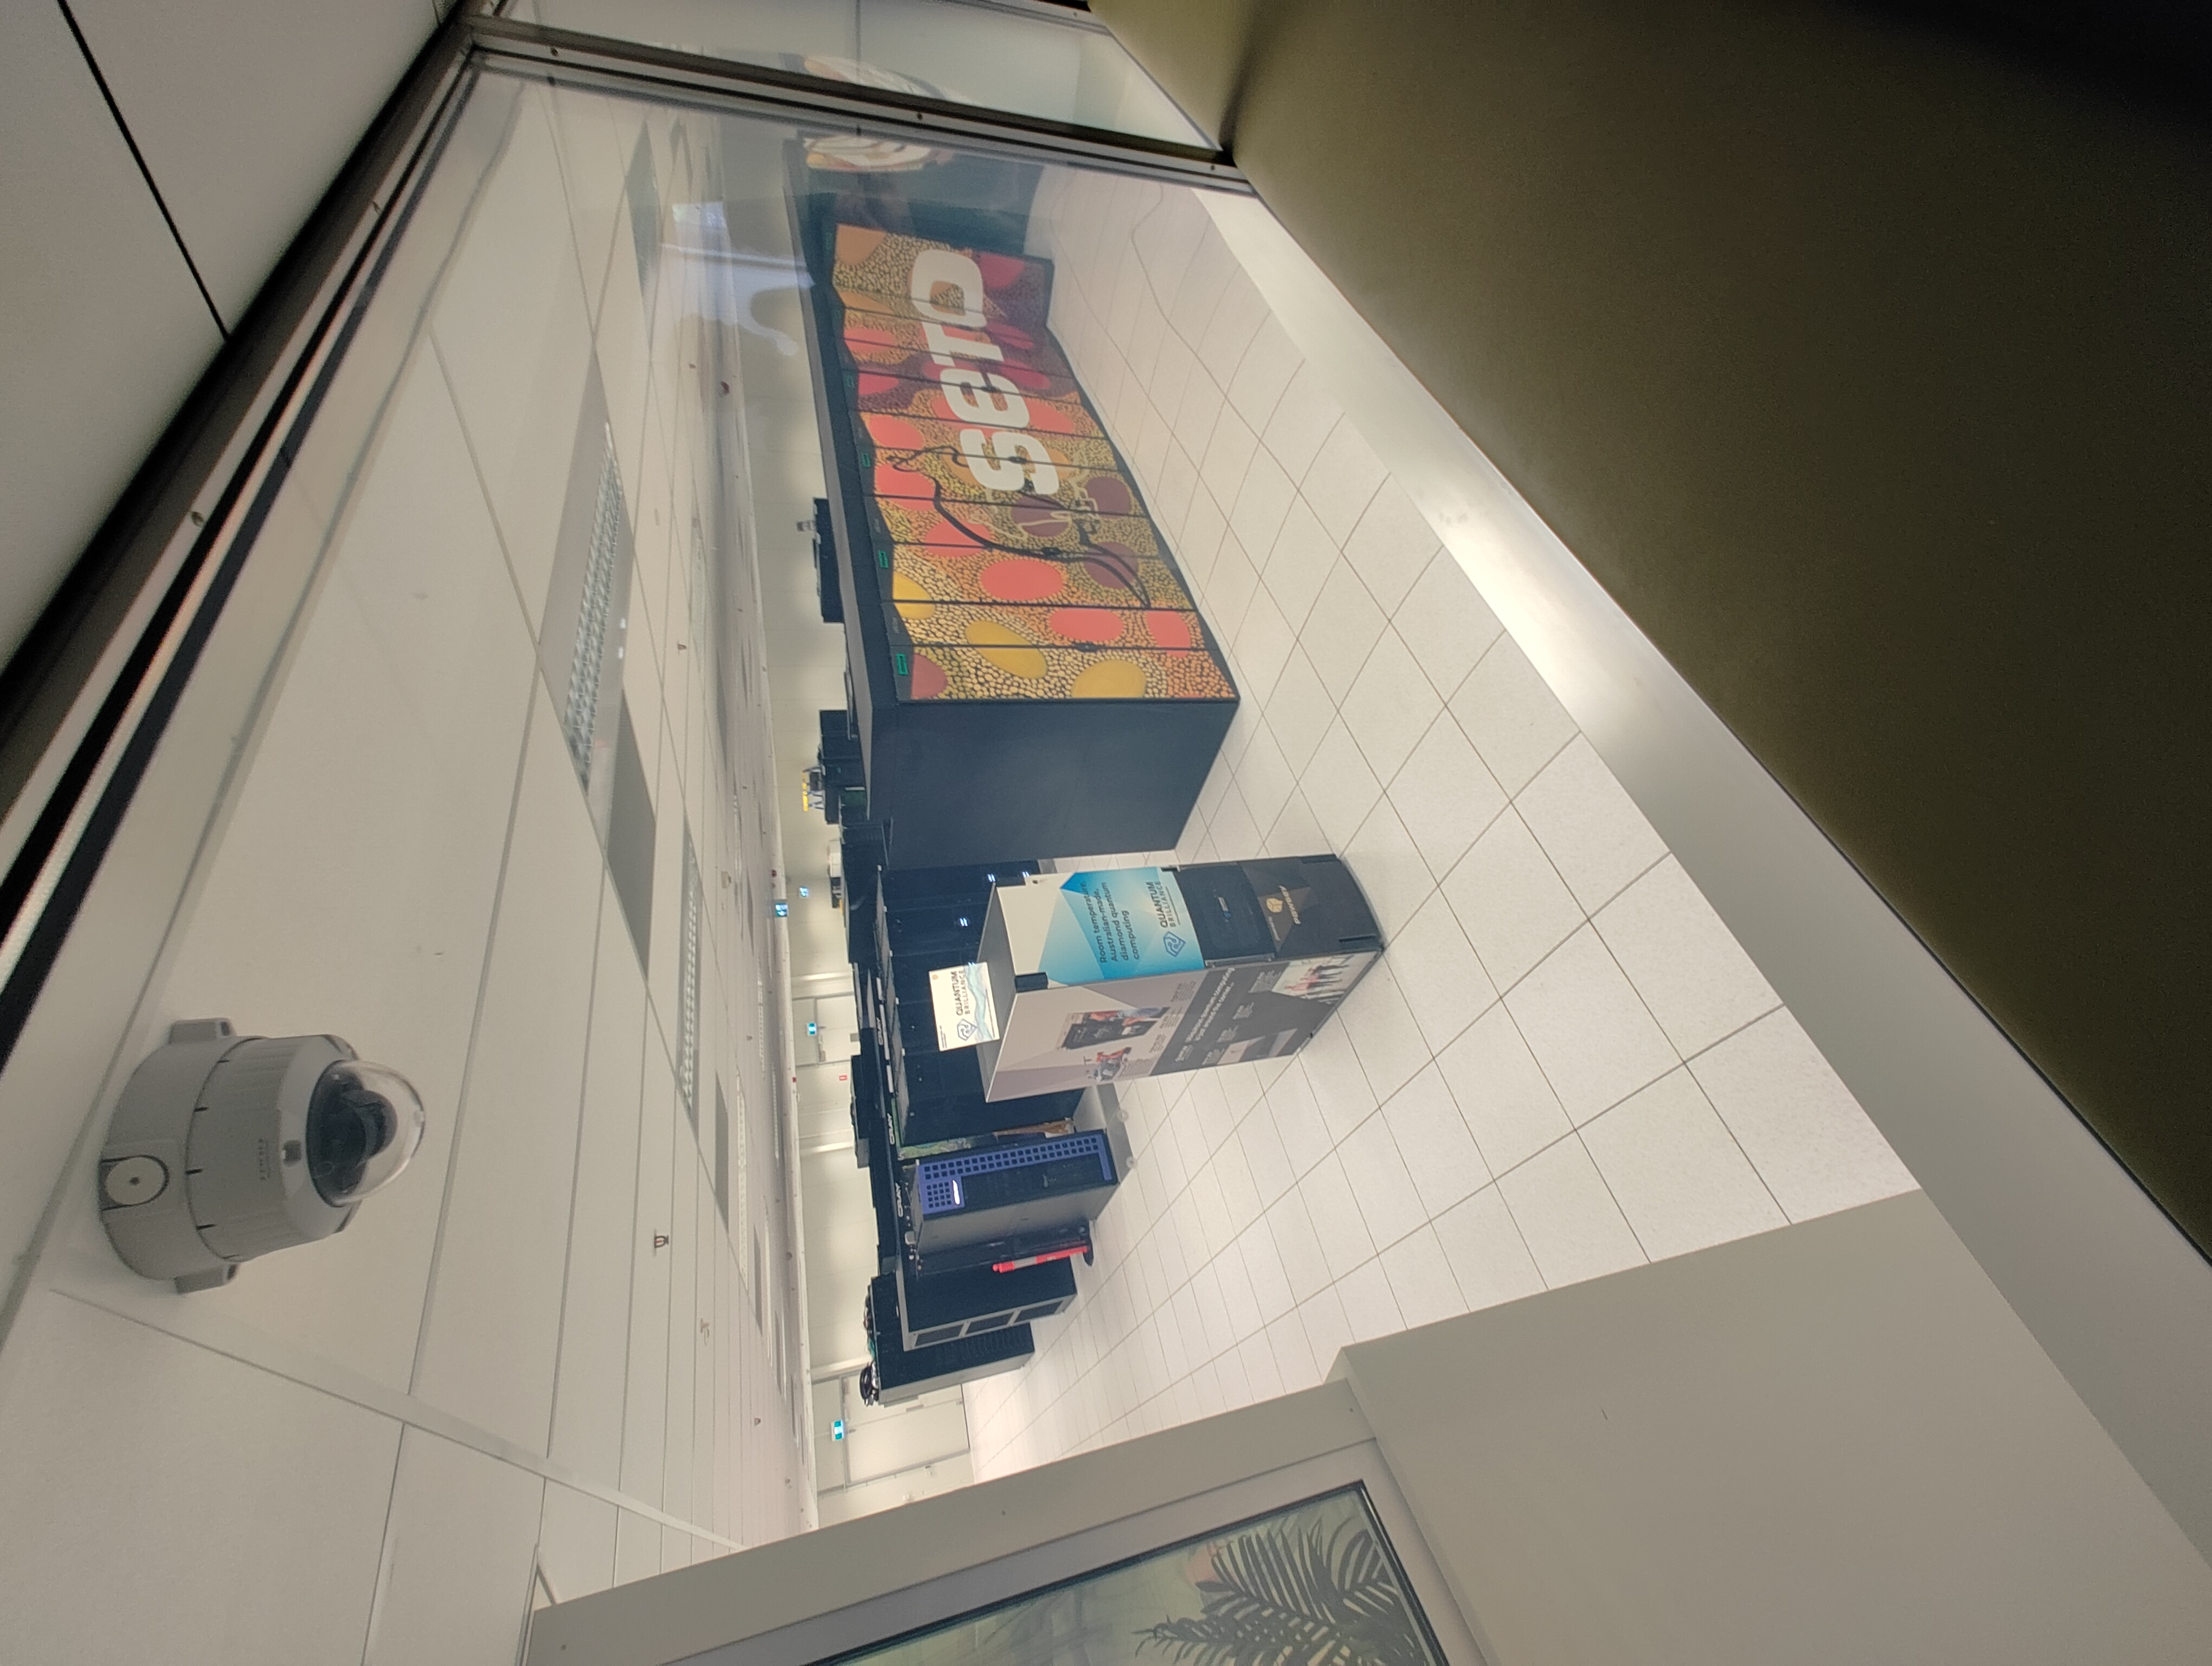
\includegraphics[height=6cm,angle=-90,origin=c]{graphics/pawsey}
  \caption{Pawsey supercomputers}
  \label{fig:pawsey}
\end{figure}
\FloatBarrier

After gazing at the black boxes that make my project possible I chatted with one of the Pawesy technicians. I'd read a recent article for a separate university unit. The article covered the consequences and worries about computer processor manufacturing in Taiwan with the current tension surrounding China trying to gain ownership of the country. With all of the processors that are necessary for the supercomputer, I asked the technician whether Pawsey has any risk mitigation or plans if issues in Taiwan escalated and crippled the worlds primary computer processor manufacturer. The conversation was short, but the technician said that the processor vendors would be directly effected and Pawesy was well equipped with stores of spare parts for the current supercomputer outfit. They mentioned that while it wasn't a current concern for Pawesy, it would be beneficial to add it to the centers discussions. I was pleased to have potentially add a possibly important point to the centers discussions. I am a stakeholder after all! While I wouldn't consider myself politically literate or focused, I think this reminds me why knowing what is going on around the world is important, even for just using a supercomputer for a university project.

\subsection{Learning a New Codebase}

It has been a challenge learning how to use and what a new codebase does. I have has to learn two main codebases that my supervisor is the author of, GPTA and dynamicEntropy (see Sections~\ref{sec:GPTA} and \ref{sec:dynaEn} for more information about them). These ase two programs that are key to performing and analysing molecular dynamics simulations. They also have lots of functionality, but only some of this has been documented so far by my supervisor. This means that sometimes things don't work and it can be difficult for me to understand why before asking my supervisor for help. I do appreciate the current documentation that is available, but for functions that have yet to be documented, I appreciate that I have access to the codebase to try and understand what is going on. While I think documentation is important for making the use of a program understood and consistent, I also see a program being free and open source equally as important. Being able to actually see what the code being run is, is important for transparency between the developer and the end user. I even found a couple of bugs when using these programs and was able to work with my supervisor to locate where in the code it was and discuss a fix. I like the collaboration that can result for open sourcing software and this would definitely be high on my list of thoughts if I write any programs for conducting computer simulations (or anything for that matter).

\subsection{SuperComputer vs. Laptop Computer}

I had to run a computer simulation for my project, but it was actually several simulations that would be run in a sequence. This was going to be orchestrated using a shell script, but a may have misheard my supervisor at some point because I thought they said I had to run this simulation on my laptop, not the supercomputer. I thought I heard that the shell script was written for the Z shell and not Bash and that the supercomputer did not have Z shell, but my personal computer did. I ran the simulation. It took three days to finish with my laptop fans and processor going full tilt. When I saw my supervisor after this, they said that running it on the supercomputer was fine, so we reran the simulation. It finished that same day. This comparison shows me the computing power difference of a laptop and a supercomputer - a lot! I already knew this, but having an unusable laptop for three days wasn't ideal when I still have things I could be doing on it. I have a new found appreciation of being able to connect remotely to a machine to complete a job or simulation and having the performance of my host machine be untouched.

\subsection{Making Mistakes}

I don't like making mistakes. Making mistakes feels like failure to me. I am slowly changing this ideology to something more positive because I have found that I get so ``in my head'' about making mistakes and asking my supervisor for help that I avoid doing the work. This is not healthy or productive. I'm glad to say that I have has a couple of good experiences when I have made mistakes in my project. One mistake that comes to mind is when I tried running a simulation without running it with any molecular dynamics parameters (the core of what the simulation is). When my supervisor found this out, they told me the fix and that was the end of it. I wasn't ridiculed or grilled for my silly mistake, I was told the solution where to go from there. Perhaps this is specific to my supervisor, but I appreciate their patience with me learning new things. I feel more comfortable with trying things or asking questions, no matter how simple, as it is just part of the learning process and isn't something to feel ashamed about.

\subsection{Supervisor Being Away}

I enjoyed the independence of my supervisor being away, but I should have engaged more with other members of the computational chemistry group to make sure I didn't get stuck on problems. I found the independence both helped me get on with my work as I knew what I had to do and it was just up to me, but also meant that I had to rely on my own motivation to achieve this. I think that my supervisor and I planned fairly well for them being away. I had a list of things to work on and the tools to do it - if I got stuck, I could get help from someone else and/or shift my focus onto some of the writing for the report (like the introduction with background from literature). I got an acceptable amount of work done during this period, but I did struggle with motivation which was disappointing. I would have liked to make some good progress and show my supervisor that I was on top of my project and had a good understanding of things. This is something I will keep in mind for honours and try to plan for if my supervisor is away and I am glad that I have experienced this now.

\subsection{Mid-Year Presentations}

I was adequately prepared for my mid-year presentation and I feel as though it went fine. I think I generally spoke clearly and covered all of the points I had in mind. With more preparation, I think I would have liked to have come up with a few more key sentences to memorise. I don't think memorising a whole talk is useful or productive, but a couple of well-thought out sentences for important parts of a talk would make it easier to follow and fill in the bits in-between with words in the moment. Public speaking is something I need to work on. I'm glad to say that I had little anxiety leading up to and during my presentation, so I see that as progress since my last time speaking. To keep the ball rolling, slide preparation and audience engagement will be important aspects for me to work in before the industry showcase at the end of the year arrives.

I was impressed by talks my peers gave. All of them were presented well and had a good grasp on the content they delivered (shown by answering audience questions). I felt privileged to hear about so many different projects across the majors that the Advanced Science program has to offer. I felt like I gained at least a small understanding over a lot of different areas of science in a short amount of time. The presentations were also a good way for me to put names to faces since joining this cohort.

\subsection{My Understanding of Chemistry}

Computer simulations are a bit different from experiments in the physical world. We can't necessarily measure things in the same way. To get values from a computer that can be compared with the real world needs important considerations about simulation design. I'm far from an expert in computer simulations or chemistry, but I have had my understanding of experiment physical chemistry challenge by stepping into the world of computer simulations. The computer simulations aren't usually attempting to replicate a real work experiment, but to simulate an environment that mimics a portion of it. I have enjoyed learning about these ideas and seeing how we can use computers in interesting ways. Interpreting the results from the simulations I have run is a challenge I am keen to tackle to show my supervisor my foundational understanding of chemistry for my final report.

\subsection{Plain Text}

I enjoy creating and utilising plain-text files for various parts of my life on my computer. I write documents, do accounting, make figures, and more, all using plain-text files. I like it because it is human-readable, simple, and can be easily version-controlled. When I stumbled across the video ``\href{https://www.youtube.com/watch?v=gd5uJ7Nlvvo}{Plain Text - Dylan Beattie - NDC Copenhagen 2022}'' I was intrigued. It's an hour-long conference talk about plain text and plain-text files - it's probably either very dull or very interesting. I'm glad that it was the latter. The speaker, Dylan Beattie, was very engaging in the topic and has other talks they have done which I might check out in the future. A large part of the talk was about the encoding of characters onto screens and into files of plain text. It's the kind of thing that's easy to overlook, but has been important in the progression of computers to today. Thanks to UTF-8 encoding, we have things like emojis with different skin tones due to different characters being able to be added to one another. This is more for accented and special characters, but for the emoji example, a seperate colour emoji added to a face in the encoding to display a face with the specified skin tone. Computers intrigue and baffle me and I think it's videos like this that elicit these conflicting feelings - something that seems simple like plain text actually being a very sophisticated system behind the scenes.

\subsection{Slumps vs. Pumps}

I have struggled throughout this year with my motivation in my university work and my project. I sometimes find it difficult to find meaning and passion in the work that I should be doing and it feels like a cloud is covering how I really feel (that I do truly enjoy this work!). These struggles also extend to my personal activities. Thankfully, I've been inspired by the great bodybuilder Arnold Schwarzenegger to strive for something called ``the pump.'' The pump is the feeling of your body being extremely strong and tight when working out and it feels great. This was what I think about when I'm struggling to be active - that I could get the pump - and it's typically the nudge I need to get back into doing physical activity that I like and makes me feel good. So, recently when I've been struggling with my work, I've considered ``the pump'' in terms of working my brain. This has helped me transition out of slumps of being unproductive to getting work done. Hard work of any kind doesn't seem attractive at first glance, so it's easy to brush it off, but just starting with something small makes it easier to continue and try and find the elusive pump.

\subsection{Thinking About Honours}

With my struggles throughout the year, I've had doubts about my ability and drive to continue on to the honours-year of my degree. Honours is a big commitment and a whole extra year of study. Being so close to having a bachelor's degree and not having a job or money at the moment makes me conscious of my position in society and expectations that I should be a good citizen and get a job as soon as possible and work until death for the greater good of the country - or something like that... I feel better that I've taken more time to think about honours and understand its importance in my academic journey. I still think I would like to be a career researcher and honours is an important stepping stone for this. I understand the challenge of honours and, despite recent struggles, I know I am capable of achieving what I want academically and I do enjoy the fight. I'm fortunate and grateful that I have so many options for next year; do honours, take the intermediate exit award and get a chemist job, take the exit award and get a job in the coffee industry, or something else I haven't considered! I think I have more or less settled on doing honours and feel confident with my choice.

\subsection{Writing Units}

I've chosen to use my elective units this year to complete two writing units. While I could be have used these units to study more chemistry, I thought that extending my writing abilities would be something useful for me as I have struggled with writing generally in different forms. Since I want to pursue a career in academia, journal article writing would be my main publishing form. I already have a decent grasp on this style of writing and understand its value in communicating scientific information to fellow researchers. However, this is a relatively small target audience, and I feel as though scientific information should be accessible to the masses to increase general understanding of the world around us and beyond. Journal articles are not always written in a way that can be well understood by a general audience. This is why I have taken these writing units, to better my skills at writing in creative non-fiction and feature article writing. These styles are more suited to general audiences and can use different techniques to get readers interested in topics they might not usually be. While I may spend most of my career writing in the scientific style required for journal articles, if I want my research to be seen by the masses, I need to know how to show them - and I think the forms I have learnt and practice as part of these units has helped significantly (so much so, that I had considerations of doing a masters degree in writing and pursuing a career through that pathway).

\subsection{New Cohort}

Having to redo NPSC3000 this year meant that I was a part of a new cohort of Advanced Science students. Previously, a change like this would have caused me significant anxiety, but I'm happy to say that this wasn't the case. A was already familiar with the Advance Science chemistry major students from this cohort, so this eased any tension I had. While I haven't has any ground-breaking chats with my fellow students, they all seem pleasant to be around and engaged with science throughout their projects. I feel as though this experience is important for building my adaptability for working with new people as I will have to join a workplace in the future and meet a new team of people (a cohort in a way).

\subsection{Generative AI}

While I don't consider myself a trend-chasing, I do like to keep an understanding in trends, typically in technology. However, with all this talk abut generative AI, I haven't found myself compelled to use it yet. I don't have any significant aversions to using services like ChatGPT, I just feel as though I haven't seen a use-case for myself and my work. I've done plenty of writing over the year, both scientific and creative, but I've relied on my own thoughts and ideas when completing these tasks. Even though using my own brain for writing can sometimes be a challenge, I feel as thought when I finally get the words down that they are authentic and mine - they're written in my voice. I see generative AI as being useful for generating code for simple programming tasks, but even then, as a novice programmer at best (that's probably still a stretch!) I would like to understand what the code means. I suppose using AI for learning to code will be useful, but complete trust and overuse could lead to bad habits and gaps in knowledge. I will continue to monitor the state of AI and consider how I might use it in my honours year next year. I see AI as a valuable tool, I just don't know how to use it effectively yet!

\subsection{Working Remotely}

This winter and autumn has been quite strange weather-wise. Cold, miserable days followed by a glimmer of warmth before more rain and cold. I'm happy to have found it possible to work from home for my project on these more miserable days when a commute under a gloomy sky to university is very unappealing. Although, it occurs to me that since I'm using the supercomputer to run my simulations remotely, my project technically doesn't need me to be present at university. However, I definitely see the value in seeing my peers and supervisor in person for quick queries, instead of sending emails back and forth. Also, I find the environment at university more conducing to getting work done which helps me with keeping on track. I'm not going to stop going to university to do my work, but it's nice to know that I can still get some things done from home if the weather is particularly miserable (or my mood for that matter). 

\subsection{Coffee Chemistry}

I see coffee as a fond hobby of mine. I enjoy learning about, talking about, smelling, brewing, and (of course) drinking speciality coffee. I'm pleased to say that my studies in chemistry have opened up new interests for me in the coffee space. Things like how a little salt in your coffee can reduce the amount of perceived bitterness when drinking it and the science being brewing the best cup of filter coffee or espresso. Brewing coffee (and cooking food in general) has similarities and benefits from using a scientific approach. Weighing ingredients and following a recipe are important for consistency and repeatability. I feel as though my training in chemistry and my interest in coffee complement each other well. I even found out about Monika Fekete, a trained PhD level chemistry with a love for coffee who has transitioned their career into the coffee industry - they're the head chemist at Breville Australia! I've tried to get into contact with Monika to ask about their journey because it is one that genuinely intrigues me.  

\subsection{Different Computer Processing Unit Technologies}

I watched the video ``\href{https://www.youtube.com/watch?v=gd5uJ7Nlvvo}{CPU vs GPU vs TPU vs DPU vs QPU}'' to learn a bit about the differences between different computer processing unit technologies. The acronyms for the different processing units are as follows:

\begin{itemize}
\item CPU - Central Processing Unit
\item GPU - Graphics Processing Unit
\item TPU - Tensor Processing Unit
\item DPU - Data Processing Unit
\item QPU - Quantum Processing Unit
\end{itemize}

The video is relatively short and briefly covers each type of processing unit, but I enjoyed it as an introduction to them. While I don't feel the need to research any of them heavily, it brought new technologies like TPU and DPU to my attention. I think more importantly, it gave me some understanding as to why my project runs its simulations mostly on the GPU. This is because my simulations are many different smalls mathematical calculations which can run in parallel on a GPU, which is what they're more or less designed for. That makes these simulations run much faster than if it were run solely on a CPU. I feel as though this project has indirectly helped me better understand computers and how they work.

\subsection{Futureness of This Research}

Something about computational chemistry feels foundational in its results. While my results I have so far are largely just values that are similar to experimental results found by someone else, I can still see my project as a contribution to research generally. It shows that the parameters to run my simulations are correct and may be used by myself or someone else in the future to run more complex simulations to make predictions on something. It's a small contribution, but I still feel proud that as an individual I was able to do something that may be important in the future.

\subsection{Sustainability of Chemistry Research}

I am always conscious of my impact that my work has on the environment. With an applied, experimental project, it is fairly simple to see your impact - you can see the waste you produce and the energy you have consumed. With this computational project, it seems a step removed from seeing the impact it has. I work on my laptop and submit simulations to be run on a supercomputer in a building I've only been to once. I can see a figure of the power consumption the Pawsey supercomputing centre requires, but for simple user like me, it almost seems like running a simulation is free. I try and get this idea out of my head quickly, because my simulations do have a resource cost that should be considered. Everything in life has an energy cost in some form and I think it is important that even though I don't directly see my energy consumption it should not be taken for granted. Perhaps in my report I could note down the number of hours of simulation time I spent to gather my results. Since I understand that my simulations do come at a cost, I make sure to check I have set it up correctly before submitting it to be run so I can minimise waste (in terms of using energy running the supercomputer to only get junk results out).

\subsection{Backing Up Big Data}

Running molecular dynamics simulations requires a lot of disk space on a computer. The largest output file is usually ta trajectory file for a simulation. It is a binary file with all of the values for the positions and velocities of particles in a a simulation for every time step. These files for my simulation are typically in the tens of gigabytes in size, so personal storage on my user on the supercomputer is quickly filled. I took it upon myself to ask my supervisor about transferring and backing up lots of data before it would become a problem. It turns out that Pawsey has a system called Banksia for storing data from discs to tape, which is a highly efficient method for storage, but comes at the cost of being slow to retrieve stored data later. Understanding has been important when backing up my data and retrieving parts of it to back up locally on a large solid-state drive that I own, for easy access. I wonder what I will do with this data once I have concluded my project. Will I keep a single copy of my whole project repository on Banksia? If so, how long will Pawsey allow it to stay there? Should I keep a copy for myself? If I keep a copy for myself, I wonder if my supervisor has strategies for archiving and/or compressing large amounts of data. Producing, using, and storing big data is a new concept for me and I'm interested in gaining knowledge in how to deal with it because I feel as though lots of data stored today is redundant, but with how cheap access to storage is, this issue doesn't seem to bother some people. It bothers me though. I wonder how much power and resources are given to storage mediums that are storing redundant data and the greater impact this could have in the future.

\subsection{Group Meetings}

At the start of my project, the computational chemistry group meetings were quite difficult for me to comprehend. I still very much enjoyed being a part of them and listening to what Curtin researchers were up to. Although the content wasn't well absorbed by me, I would still jot down interesting words and topics that came up in meetings, so that I could search them up later in my own time and try gain a better understanding. As my project progressed and I started to learn more about computational chemistry, I noticed that I could pick out more and more ideas that were presented in the meetings. It felt really good to see my understanding validated silently. I felt a bit more of an outsider in the earlier meetings because of my lack of knowledge in this space, but I'm pleased to say that I feel like part of the group now in terms of my understanding of computational chemistry. There is still lots to learn, but my foundational knowledge feels strong enough to ask more questions and interact in these meetings going forward.

\subsection{Supervisor Report}

I feel as though the supervisor report I received (Appendix~\ref{appendix:suprep}) is an accurate reflection of may capabilities from this year. It suggests that I am proficient with my use of technology and I'm glad this was seen. I flagged that my communication and teamwork skills were developing in my self assessment and these were identified as still developing by my supervisor. I can understand this as I've still has some anxiety issues which get worse when I get in a slump of not being productive. I think I have made progress in this space, but can see this being something I need to push towards being better and get out of my comfort zone, going into honours. Some of my planning stayed in the developing stage - another key skill for honours. I still finding ways that suit my workflow for planning my studies, as well as my personal life. I sometimes get distracted by finding ``the best way'' of planning, but really I just need to find something that works well enough and stick to it - I think this is what has been holding me back. Overall, I am happy with the report I received and I feel comfortable in asking for advice by my supervisor in regards to developing my skills and I'm proud of the rapport I have built with my supervisor.

\section{Resources}

The following are descriptions of some of the key resources I have utilised in my project.

\subsection{Pawsey}

The Pawsey Supercomputing Centre is integral to running computationally intense molecular dynamics computer simulations. Without it, the scale of my project would be drastically smaller. I have used a GPU enabled virtual machine to run a large number of my simulations. Similarly, I have used the Topaz machine with its GPU nodes. The code used for the simulations is optimised for running on GPUs, so these machines have been well suited for the task. The Banksia service has been used to back up the large amounts of simulation data I have produced over the course of the project. I will acknowledge Pawesy in my final report providing these resources to complete this project.

\subsection{GPTA}
\label{sec:GPTA}

This is a publicly available program written by my supervisor in Fortran for analysing trajectory data from molecular dynamics simulations - \href{https://github.com/praiteri/GPTA}{GPTA} stands for General Purpose Trajectory Analyser. This package has been important for interpreting results from simulations.

\subsection{DynamicEntropy}
\label{sec:dynaEn}

This program was written by my supervisor and is not currently available to the public, but I believe it will be when the accompanying documentation is finished being written. The program is a python module that acts as a wrapper for the open source computational chemistry code, \href{https://github.com/openmm/openmm}{OpenMM}. I appreciate the work my supervisor has put into this program as it acts as an approachable way of running simulations using the complex and useful OpenMM project. The program also has some functionality for analysing simulations too, which has been used for my project.

\section{Peer Reviews}

\subsection{Reviews Given}

The following section contains the verbatim body text of emails sent to my peers after reviewing their portfolios.

\subsubsection{Stefan Hofmann}

Overall, I think your portfolio is well-structured and rich with content. I like the use of hyperlinks, screenshots, code-blocks and other media - I think it makes your portfolio appear "weighty" and interesting. The use of different headings and markup elements make pages easy to follow. Some pages, such as "Test Server," with less information could perhaps be merged with another page to cut down on blank-looking space in the portfolio.

A page I looked at more was "ML Model - Literature Review." I think this page (and section it was a part of) is extremely well done. I was able to read along easily - your summaries of papers made it simple for a non-computer science student to understand the gist of things. Appropriate referencing is always good to see. Having a conclusion to your literature review was a nice way to show your learning and the importance of conducting the review.

\subsubsection{Samuel Cunningham}

Overall, I think your portfolio is concise and well put-together. I like the variety of media you have included in project-related sections. I would have liked to have more media present in your reflections, but I do like that you have dated them. This gives it a chronology to follow which works well for seeing progression and your thoughts going through the year (perhaps not adding additional media to the reflections after they were written leaves them as appearing more genuine and in the moment which I can see working also).

I had a closer look at the "AI Advancements" section and I think it is a great example of your capabilities in your field. I'm not usually so inclined to think about entrepreneurship, but reading through this section was inspiring. I'm not running out to start a company right now, but I'm glad to see my peers doing well in this space and I will have this in the back of my mind going forward. This section presents really well and I like the media and ideas you've included.

\subsubsection{Rahul Sinha}

Overall, I think your portfolio is a solid repository of information for your project. I like the extensive use of links throughout and especially within the table on the "Research" page - if only I had used some tables in my portfolio! The sectioning and inclusion of information is logical and concise. I like that your reflections are dated, I think that this gives a nice timeline for your learning and feelings going through the year. 

A had a closer look at the page "Reflection 09-03-2023." This reflection flows well and I can see your thought process and attempt at applying what you had learnt from that weeks Advanced Science class. I appreciate your honesty and feelings about your learning in your other classes. I think it was a good standard for what I reflection should be like.

\subsubsection{Thomas Munyard}

This reflection [Reflection 15: Project meeting in the midst of chaos] is well detailed and has an excellent narrative quality to it. There is a great balance between personal thought, description of events, and your learning. I appreciate the introspection and honesty you have put into the reflection for others to read - I think many students will relate to what you've said. Giving the reflection a unique title is also a nice detail for this polished piece.

\subsubsection{Claudio Pedrick}

Overall, your portfolio is concise and well put together. I like the pages about yourself and your project. They make the rest of the portfolio more approachable by giving a clear background. Dating your reflections gives a nice sense of progression and chronology to them and the accompanying titles make them unique. 

I had a closer look at the reflection, "S2:Wk9 - Yeh… So I definitely Jinxed it." I like the personality you write with and the honesty you show with your feelings. As I'm also using Pawsey resources, I resonated with your aversion to seeing emails from David Schibeci. This reflection has good description and flows nicely too.

\subsection{Reviews Received}

The following section contains the verbatim body text of emails received from my peers after reviewing part of my portfolio.

\subsubsection{Thomas Munyard}

Reading this reflection [Pumps vs. Slumps], I found myself thinking back throughout the year when I have been in the exact same mindset as you spoke of in the first few sentences. This year has been an extreme struggle and my motivation also dwindled throughout the year with it being extremely hard to force myself to continue to move forward due to a number of different reasons.  
 
I have really found this analogy of 'the pump' very insightful and I believe that I will also try to incorporate this into my mindset as you have done. I think it is very important to remember how important exercise is and how it can help not just physically but also mentally. It is amazing to then think how this can be applied to our brain in order to complete our work.  
 
In order to improve this reflection, I think it could be useful to potentially include a precise example throughout the year when you have been struggling to find motivation and reflect on what you have done to achieve this desired 'pump'. It is then important to reflect on how this is developing you professionally as this reliance and perseverance is very important when you go into a job. There will be tasks which you don't want to necessarily complete, but through developing this mindset through your studies, you will have the tools in order to persevere and finish the job. 
 
Overall, I thoroughly enjoyed this reflection as it was very different from previous reflections I had previously read. I wish you all the best for the rest of the year! 

% \printbibliography

\appendix

\section{Supervisor Report}
\label{appendix:suprep}

Please see the following page for the supervisor report.

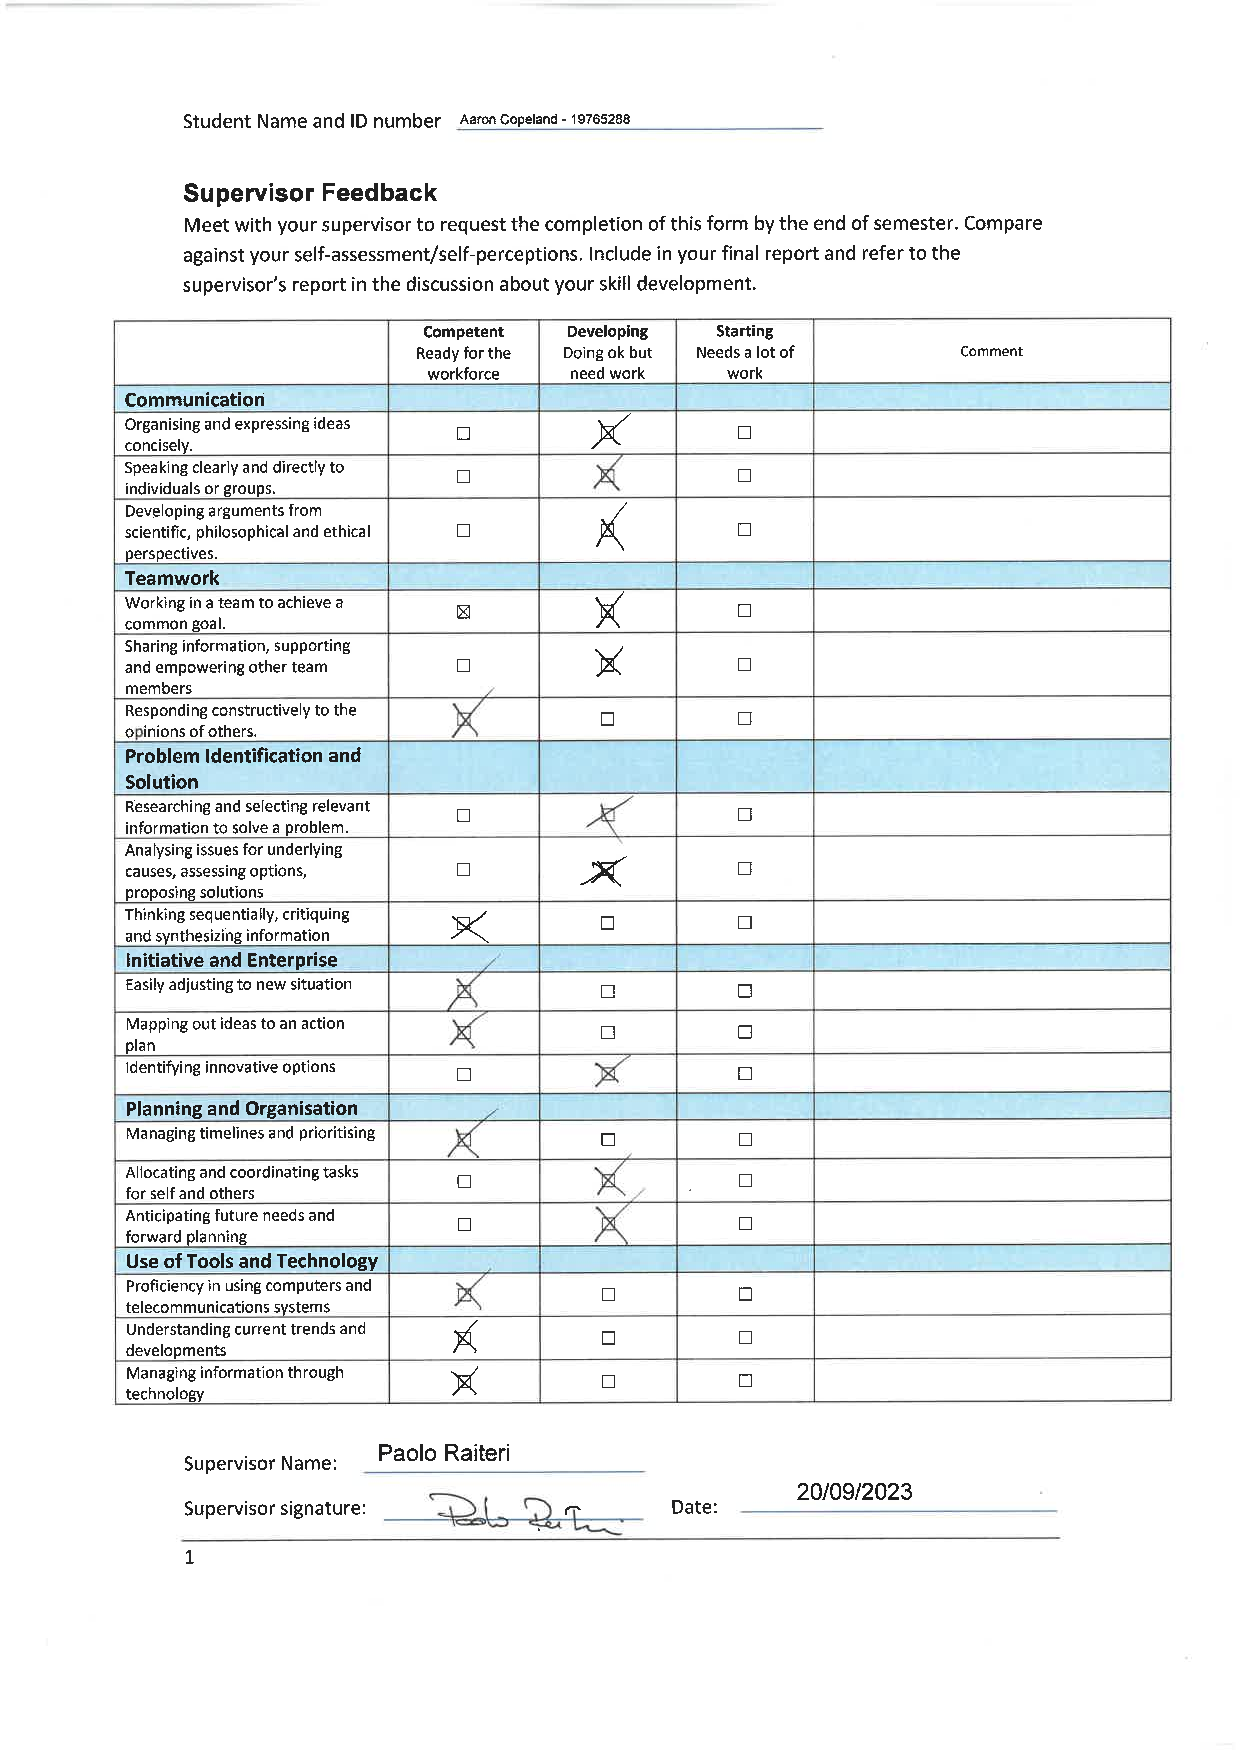
\includepdf[pages=-]{graphics/suprep.pdf}

\end{document}